% Theme selection
\usefonttheme{professionalfonts}
\useinnertheme{circles}
\usecolortheme{whale}
\usecolortheme{orchid}

% Outer theme
% Footline: Title, Author ... Page Number
% Headline: Sections with navigation circles
\useoutertheme{miniframes}
\defbeamertemplate*{footline}{my page number}{%
    \begin{beamercolorbox}[colsep=1.5pt]{upper separation line foot}
    \end{beamercolorbox}
    \begin{beamercolorbox}[ht=2.5ex,dp=1.125ex,%
      leftskip=.3cm,rightskip=.3cm plus1fil]{title in head/foot}%
      \leavevmode{\usebeamerfont{title in head/foot}\insertshorttitle, %
                  \usebeamerfont{author in head/foot}\usebeamercolor[fg]{author in head/foot}\insertshortauthor}%
      \hfill%
      {\usebeamercolor[fg]{title in head/foot}%
       \usebeamerfont{title in head/foot}%
       \insertpagenumber\,/\,\insertpresentationendpage}%
    \end{beamercolorbox}%
    \begin{beamercolorbox}[colsep=1.5pt]{lower separation line foot}
    \end{beamercolorbox}
} 
\setbeamertemplate{footline}[my page number]

\defbeamertemplate*{headline}{my head theme}
{%
  \begin{beamercolorbox}[colsep=1.5pt]{upper separation line head}
  \end{beamercolorbox}
  \begin{beamercolorbox}{section in head/foot}
    \vskip2pt\insertnavigation{\paperwidth}\vskip2pt
  \end{beamercolorbox}%
  \begin{beamercolorbox}[colsep=1.5pt]{lower separation line head}
  \end{beamercolorbox}
}
\setbeamertemplate{headline}[my head theme]

\usepackage{remreset}
\makeatletter
\@removefromreset{subsection}{section}
\beamer@compresstrue
\makeatother
\setcounter{subsection}{1}

% additional packages
\usepackage{soul,array,booktabs,longtable,xcolor,colortbl,textcomp,%
            calc,multicol,ragged2e,makeidx,xspace,%
            csquotes}

% bibliography
\usepackage{natbib}            
\bibliographystyle{alpha}

% language
\usepackage[english]{babel}
\usepackage[english]{varioref}
\selectlanguage{english}

% fonts
\usepackage{fontspec}
\defaultfontfeatures{Scale=MatchLowercase,Ligatures=TeX} 
\setromanfont[Numbers=Lining,%
              BoldFont={MinionPro-Semibold}]{Minion Pro} 
\setsansfont[ItalicFont={MetaPro-BookItalic},%
             Numbers=Lining]{MetaPro}
\setmonofont[BoldFont={LucidaSansTypewriterStd-Bd},%
             ItalicFont={LucidaSansTypewriterStd-Obl},%
             BoldItalicFont={LucidaSansTypewriterStd-BOb}]
            {LucidaSansTypewriterStd}
\usepackage[small]{eulervm}

% math
\usepackage{amsmath,amssymb}

\theoremstyle{definition}
\newtheorem{mytheorem}{\iflanguage{english}{Theorem}{Satz}}
\newtheorem{mycorollary}[mytheorem]{\iflanguage{english}{Corollary}{Korollar}}
\newtheorem{mylemma}[mytheorem]{\iflanguage{english}{Lemma}{Lemma}}
\newtheorem{mydeflemma}[mytheorem]{Definition + Lemma}

\theoremstyle{definition}
\newtheorem{mydefinition}[mytheorem]{Definition}

\theoremstyle{remark}
\newtheorem{myremark}[mytheorem]{\iflanguage{english}{Remark}{Bemerkung}}
\newtheorem{myexample}[mytheorem]{\iflanguage{english}{Example}{Example}}

% some abbreviations
\newcommand{\code}[1]{\texttt{\small#1}}
\newcommand{\acronym}[1]{\textsc{\MakeLowercase{#1}}}
\renewcommand{\emph}[1]{\textbf{#1}}
\newcommand{\myN}{\mathbb{N}}
\newcommand{\myZ}{\mathbb{Z}}
\newcommand{\myR}{\mathbb{R}}
\newcommand{\myC}{\mathbb{C}}
\newcommand{\myP}{\mathbb{P}}
\newcommand{\OO}{\mathcal{O}}

% indexing
\makeindex

% spacing issues
\usepackage[thinspace,thinqspace,squaren,textstyle]{SIunits}
\newcommand{\szb}{\mbox{z.\,B.}\xspace}
\newcommand{\sia}{\mbox{i.\,Allg.}\xspace}
\newcommand{\sdh}{\mbox{d.\,h.}\xspace}
\newcommand{\szz}{\mbox{z.\,Z.}\xspace}
\newcommand{\sie}{\mbox{i.\,e.}\xspace}
\newcommand{\seg}{\mbox{e.\,g.}\xspace}

% pdf and references
\hypersetup{
  pdfproducer={\myname},
  pdfcreator={\myname},
  pdfkeywords={\mykeywords},%
  pdfstartview=FitH,%
  pdfpagemode=UseOutlines,%
  bookmarksopenlevel=2}

% Meta data
\title{\mytitle}
\author[\myname]{\\[-1em]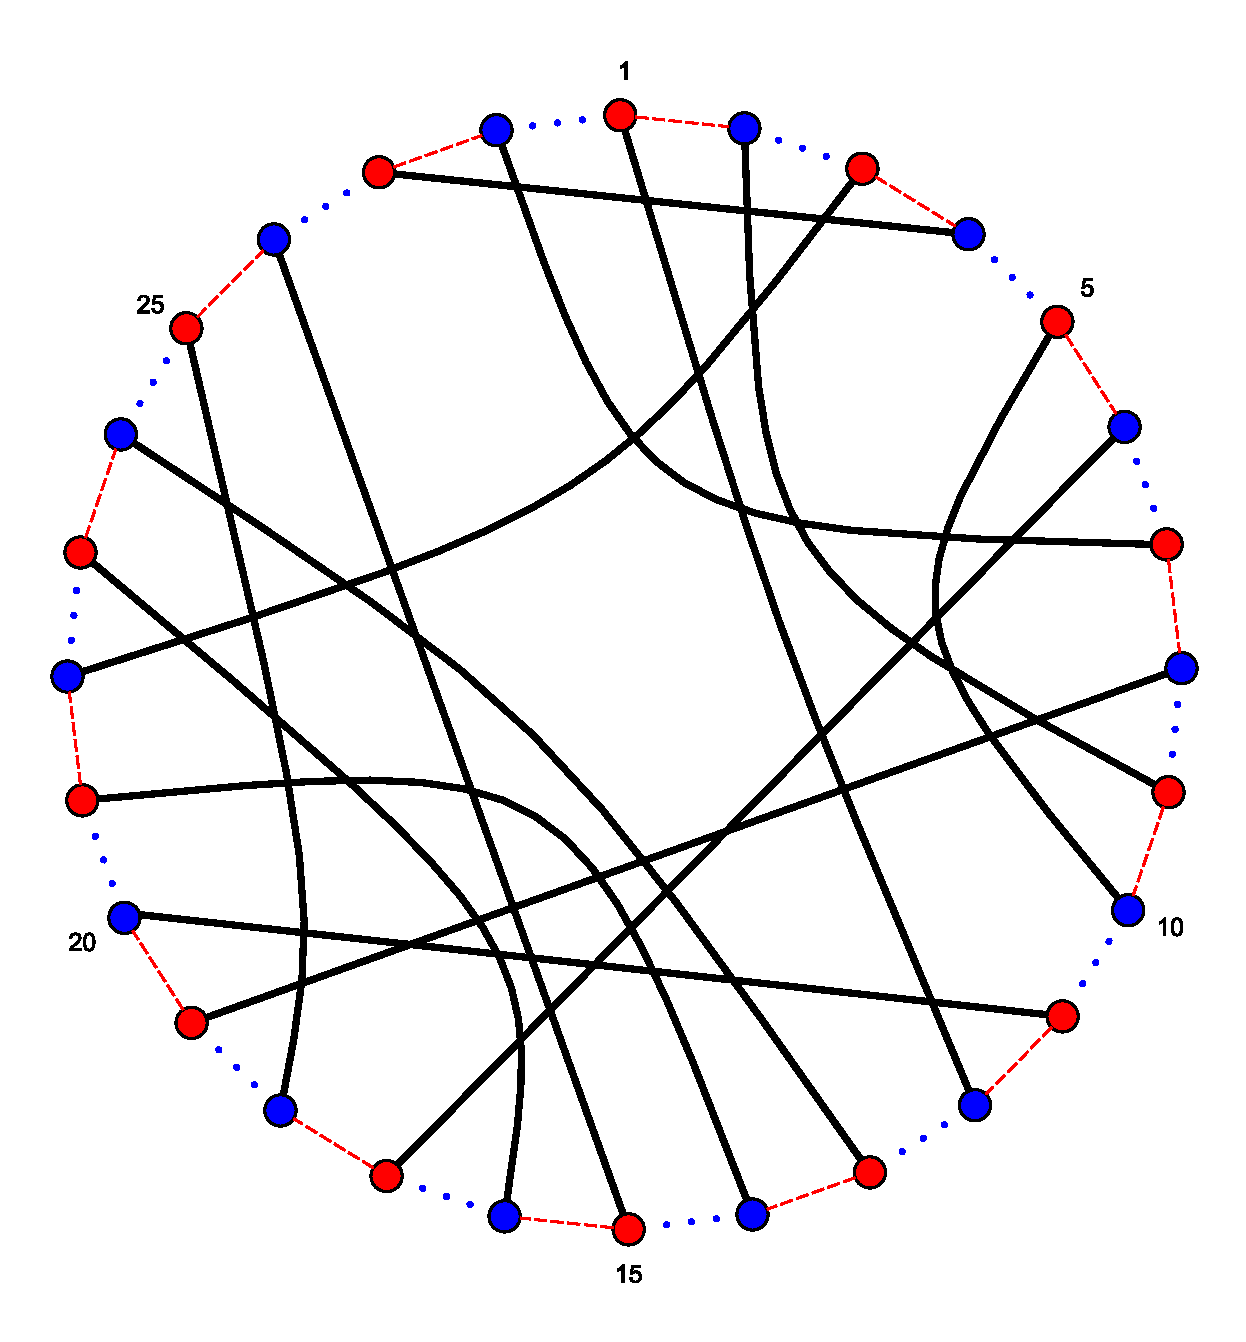
\includegraphics[width=0.45\textwidth]{../thesis/figures/two_cycles.eps}\\\myname, \mydate\vspace{-1em}}
\date{}
\subject{\mytitle}
\institute{\myinstitute}
  
% Graphics
\usepackage{color,tikz}
\usetikzlibrary{svg.path,calc,decorations.pathreplacing}
  
% listings and pseudocode
\usepackage{listings}
\lstset{basicstyle=\scriptsize\ttfamily,numbers=left,%
  numberstyle=\tiny\ttfamily,%
  stepnumber=1,%
  language=C++}%
\usepackage{algorithm2e}

% Pseudocode definition
% Algorithm2e
\SetAlFnt{\scriptsize\sf}
\SetKw{KwRet}{return}
\LinesNotNumbered
\DontPrintSemicolon

\newcommand{\myalgosize}[1]{#1}

\newcommand{\mycomsty}[1]{\myalgosize{\textsf{#1}}}
\SetCommentSty{mycomsty}
\newcommand{\mykwsty}[1]{\myalgosize{\textbf{\textsf{#1}}}}
\SetKwSty{mykwsty}
\newcommand{\myargsty}[1]{\myalgosize{\textit{\textsf{#1}}}}
\SetArgSty{myargsty}
\newcommand{\myfuncsty}[1]{\myalgosize{\textsf{#1}}}
\SetFuncSty{myfuncsty}

% Epigraphs
\usepackage{epigraph}
\setlength{\epigraphwidth}{0.8\textwidth}

% Theorems
%\setbeamercovered{transparent}
%\setbeamertemplate{theorems}[numbered]

\AtBeginSection[]
{
   \miniframesoff
   \begin{frame}
       \frametitle{\iflanguage{english}{Contents}{Gliederung}}
       \tableofcontents[currentsection]
   \end{frame}
   \miniframeson
}